\documentclass[11pt, oneside]{article}   	% use "amsart" instead of "article" for AMSLaTeX format
\usepackage{tabu}
\usepackage{geometry}                		% See geometry.pdf to learn the layout options. There are lots.
\geometry{letterpaper}                   		% ... or a4paper or a5paper or ... 
%\geometry{landscape}                		% Activate for rotated page geometry
%\usepackage[parfill]{parskip}    		% Activate to begin paragraphs with an empty line rather than an indent
\usepackage{graphicx}				% Use pdf, png, jpg, or eps§ with pdflatex; use eps in DVI mode
								% TeX will automatically convert eps --> pdf in pdflatex	
								
\usepackage{amssymb}
\usepackage{textcomp}
\usepackage{ragged2e}
\usepackage{graphicx}

\usepackage{listings}
\lstset{numbers=left,tabsize = 1,language=python}
\graphicspath{ {images/}}
%SetFonts

%SetFonts


%\title{CSCI 5352 Problem Set 1}
%\author{Donovan Guelde}
%\date{}							% Activate to display a given date or no date

\begin{document}
%\maketitle
\begin{flushright}
Donovan Guelde\\
PS1\\
CSCI 5352\\
\end{flushright}
\justify
1.a. where A\textsubscript{i,j} = 1 implies that there is an edge from node j to node i 
\vskip.1in

\begin{tabu} to 0.4\textwidth { |X[c] |X[c]|X[c]|X[c] |X[c]|X[c]|}
	\hline
	 & 1 & 2 & 3 & 4 & 5 \\
	\hline
	1 & 0 & 0 & 1 & 1 & 0 \\
	\hline
	2&1&0&0&0&0  \\
	\hline
	3&0&1&0&0&1 \\
	\hline
	4&0&0&0&0&1 \\
	\hline
	5&1&0&0&1&0 \\
\hline
\end{tabu}\\
\justify
\bigskip\bigskip
1.b.\\
	\indent 1\textrightarrow \{2,5\}\\
	\indent 2\textrightarrow \{3\}\\
	\indent 3\textrightarrow\{1\}\\
	\indent 4\textrightarrow\{1,5\}\\
	\indent 5\textrightarrow\{3,4\}\\
	

\justify
1.c. \(top, dark\ nodes\)
\vskip.1in
\begin{tabu} to 0.4\textwidth { |X[c] |X[c]|X[c]|X[c] |X[c]|X[c]|}
	\hline
	 & 1 & 2 & 3 & 4 & 5 \\
	\hline
	1 & 0 & 1 & 1 & 1 & 1 \\
	\hline
	2&1&0&1&1&1  \\
	\hline
	3&1&0&0&0&0 \\
	\hline
	4&1&1&0&0&0 \\
	\hline
	5&1&1&0&0&0 \\
\hline
\end{tabu}\\
\justify


 \(lower, light\ nodes\)
\vskip.1in
\begin{tabu} to 0.4\textwidth { |X[c] |X[c]|X[c]|X[c] |X[c]|X[c]|}
	\hline
	 & 1 & 2 & 3 & 4 & 5 \\
	\hline
	1 & 0 & 1 & 1 & 1 & 1 \\
	\hline
	2&1&0&1&1&1  \\
	\hline
	3&1&0&0&0&0 \\
	\hline
	4&1&1&0&0&0 \\
	\hline
	5&1&1&0&0&0 \\
\hline
\end{tabu}\\

\bigskip\bigskip
\justify
2.a. k = A1\\
2.b.  m = $k^T$[1]\\
2.c.  N = [$A^2$]\\
2.d.  \#triangles = trace([$A^3$])

\bigskip
\bigskip
\justify
3.  For one partition of a  bipartite network, mean degree c = m/n.  We eliminate the 2 from the familiar formula c=2m/n because only one end of an edge connects with one node in each partition.  This leads to:\\
\indent 
$c_1 = m/n_1$\\
\indent 
$c_2 = m/n_2$\\
where m is the number of edges in the bipartite graph.  m carries the same value in each expression.  So:\\
$m=c_1n_1$\\
$m=c_2 n_2$\\
$c_1n_1 = c_2n_2$\\
$c_2 = (n_1/n_2) c_1$\\

\bigskip
\bigskip
\justify
4.a.\\
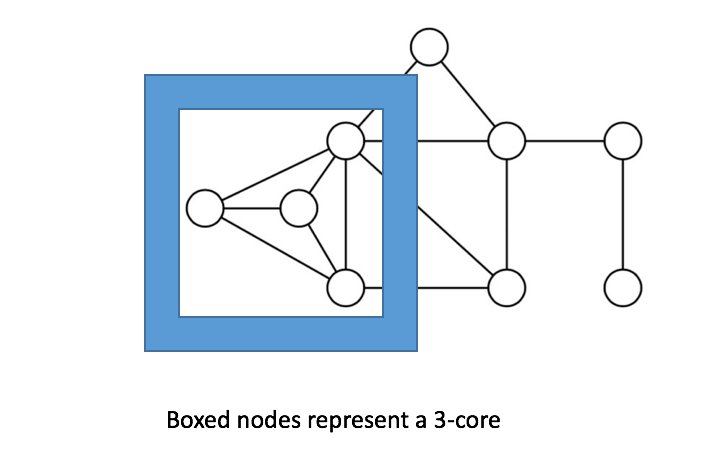
\includegraphics{3core}\\
\vskip 1in
\justify
4.b. $$reciprocity = (1/m)\sum_{ij} A_{ij} A_{ji}$$
\center = (1/8)(1+1+1) = 3/8
\justify
4.c.  cosine similarity of vertices A and B in network (C) = \[ \frac{2}{\sqrt{4*5}}\  = \frac{1}{\sqrt{5}} \]\\
\justify
5. Proof: \\
\indent
Prove by induction that
\center(1) $n=k(k-1)^{d-1}$\\
\justify
\indent
\indent
vertexes can be reached in d steps, where d is a natural number.\\
\\
Base Case:\\
\indent When d=1, k nodes are reachable.  This follows from the structure of a Cayley tree.\\
\indent From the root node, exactly k nodes are reachable in 1 step.  So, when d=1,\\
\center $n=k(k-1)^{d-1} = k(k-1)^{0} = k$\\
\justify
\indent
\indent For d=2, $n=k(k-1)^1$, since each node connects to exactly k nodes, inclusive of parent\\
\indent and offspring.  In other words, every additional step from root node results in n=n(k-1)\\
\indent reachable nodes.\\
Induction Step:\\
\indent Let s be any real number greater than 1, and suppose (1) above holds for d = s. Then:\\
\center $n=k(k-1)^{s}$\\
\justify
\indent for s=s+1:\\
\center $n(k-1) = k(k-1)^{(s+1)}$\\
\[ n = \frac{k(k-1)^{s+1}}{k-1}\]
$n = k(k-1)^s$\\
\justify
\indent Thus (1) holds for s = d+1\\

\justify
Conclusion:\\
\indent
By the principal of induction, (1) is true for all d st d is a natural number greater than\\
\indent or equal to one.\\
\justify
Diameter of a Cayley tree is a path from one leaf through the root to any other leaf with no repeating nodes.  Diameter = 2*radius+1 = (2(n-1)/k) +1 where n = total number of nodes in the tree, as opposed to reachable nodes as used in proof above.\\
\\
Cayley trees do exhibit the "small-world" effect. As stated above, the diameter = (2(n-1)/k)+1, and the number of new nodes as the diameter increases = $k(k-1)^{d-1}$\\
This means that the number of nodes n must increase by $k(k-1)^{d-1}$ in order to increase diameter by 1.  \\
So: $\Delta n = k(k-1)^{d-1}$\\
\indent log$\Delta n = (d-1)log(k(k-1))$\\
\indent $(d-1) = \frac{log \Delta n}{log(k^2 - k)}$\\
\indent $d = \frac{log \Delta n}{log(k^2 - k)} + 1$\\
As n grows larger, diameter d grows as a factor of log(n)\\
\\

\justify
6.a.  $MND = (1/2m)\sum_{uv}^{n} k_vA_{uv}$\\
\indent $= (1 /nk_{average} )\sum_{uv}^{n}k_vA_{uv}$\\
\indent where $\sum_{uv}^{n}k_vA_{uv}$ is the equivalent of matrix multiplication AA, resulting in:\\
\indent $MND = (1/nk_{average})\sum{uv}A^2$ where $\frac{\sum A^{2}}{n} = k_{average}^2$\\
\indent $=\frac{n k_{average}^{2}}{nk_{average}}$\\
\indent $=\frac{k_{average}^2}{k_{average}}$\\
\\
\vskip2in
6.b.\\
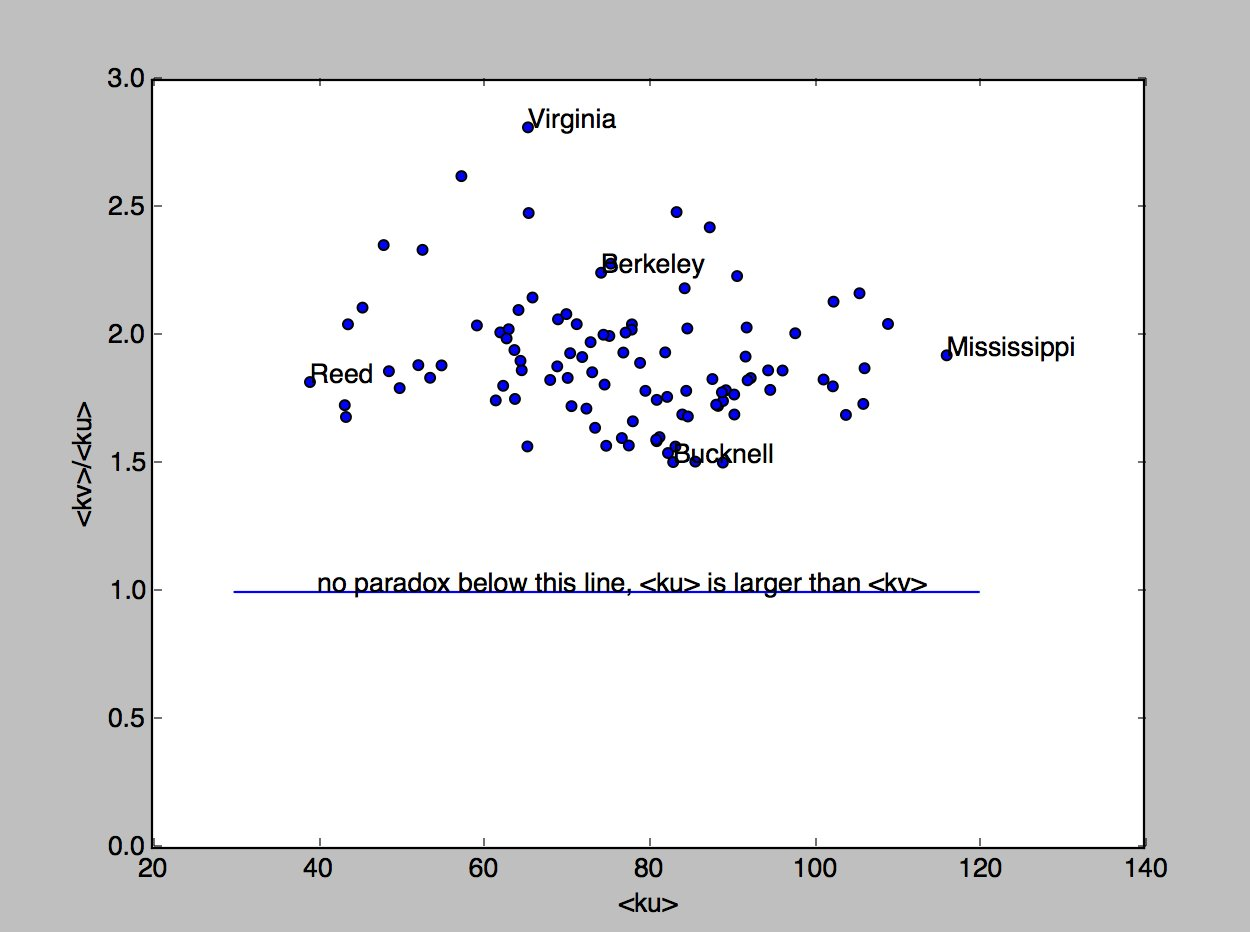
\includegraphics[scale=.5]{FB100}\\
Considering the similarity of the networks in question, as well as their sizes, it is not too surprising that all of the networks included in the dataset exhibit the 'Friendship Paradox.'  The <kv>/<ku> value appears to be centered around 1.5 to 2, regardless of other network factors, so there does not appear to be a dependency between MND and mean degree.\\
\\
6.c. The majority illusion is closely related to the friendship paradox.  Considering that, on average, our friends have more friends than we do, many of our friends may be extremely popular hubs in the network, rather than members with an average number of connections.  Since the same idea applies to all members of a given network, a random distribution of network members exhibiting property x may cause the majority illusion if, by chance, some of these property-x exhibiting members are also popular hub nodes.  While q (the fraction of vertices exhibiting property x) may be low, the probability of a given vertex being connected to a vertex exhibiting x may be high.\\
\\
\\
\\
\\
\\
\\
\\
\\
\\

\begin{lstlisting}
# Author: Donovan Guelde
# CSCI 5352 PS1
# references: online documentation for numpy
# Collaborators: None

import numpy as np
import os



class Network:
	def __init__(self,fileName):
		self.n = 0
		self.kAverage = 0
		self.degreeVector=[]
		self.associationMatrix = self.readFile(fileName)
		self.m = np.sum(self.associationMatrix)/2
		self.mnd = self.getMND()
	def readFile(self,fileName):
		with open("./CSCI5352_Data/facebook100txt/"+fileName+"_attr.txt",'r') as f: 
		#uses attr file to initialize a 2d matrix of appropriate size
			counter=0
			for line in f:
				counter+=1
			associationMatrix = np.empty((counter,counter))
			self.n = counter-1 #-1 for label row
			associationMatrix.fill(0)
		f.close()
		with open("./CSCI5352_Data/facebook100txt/"+fileName+".txt",'r') as f: 
		#uses data file to build association matrix (assumes simple graph)
			lines = f.readlines()
			for line in lines:
				line = line.split()
				associationMatrix[int(line[0])][int(line[1])] = 1 
				#make it undirected...
				associationMatrix[int(line[1])][int(line[0])] = 1
		f.close()
		self.degreeVector = np.sum(associationMatrix,axis=0)
		kAverageSum=0
		for index in range (1,self.n+1): 
			
			kAverageSum += self.degreeVector[index]
		self.kAverage = kAverageSum/self.n
			
		return associationMatrix
	def getMND(self):
		associationMatrixSquared = np.linalg.matrix_power(self.associationMatrix,2)
		self.mnd = (np.sum(associationMatrixSquared)/np.sum(self.associationMatrix))
		return self.mnd

def main():
	plotArray=np.empty((100,2)) #an array of points to plot
	nameArray=[""]*100 
	#array to hold names of schools where [index] corresponds to plotArray[index]
	nextUniversity = [2]
	lastUniversity = [2]
	counter=0
	for file in os.listdir("./CSCI5352_Data/facebook100txt/"):
		if (file != ".DS_Store"):
			
			nextFile, fileExtension = os.path.splitext(file)
			nextUniversity = nextFile.split('_')
			if (str(nextUniversity[0]) != str(lastUniversity[0])):
				nextGraph = Network(nextUniversity[0])
				plotArray[counter][0] = float(nextGraph.mnd)
				plotArray[counter][1] = float(nextGraph.kAverage)
				
				nameArray[counter] = str(nextUniversity[0])
				print nameArray
				lastUniversity=nextUniversity
				counter+=1
	np.savetxt("plotResults.txt",plotArray)
	with open("nameResults.txt","w") as f:
		np.savetxt(f,nameArray,fmt='%s')

main()
\end{lstlisting}




\end{document}  